%%%% Better Poster latex template example v1.0 (2019/04/04)
%%%% GNU General Public License v3.0
%%%% Rafael Bailo
%%%% https://github.com/rafaelbailo/betterposter-latex-template
%%%% 
%%%% Original design from Mike Morrison
%%%% https://twitter.com/mikemorrison

\documentclass[a0paper,fleqn]{betterposter}
\usepackage{xcolor}
\usepackage[most]{tcolorbox}
\usepackage[export]{adjustbox}


%%%% Uncomment the following commands to customise the format

%% Setting the width of columns
% Left column
\setlength{\leftbarwidth}{0.17\paperwidth}
% Right column
\setlength{\rightbarwidth}{0.29\paperwidth}

%% Setting the column margins
% Horizontal margin
\setlength{\columnmarginvertical}{0.05\paperheight}
% Vertical margin
% \setlength{\columnmarginhorizontal}{0.15\paperheight}
% Horizontal margin for the main column
\setlength{\maincolumnmarginvertical}{0.05\paperheight}
% Vertical margin for the main column
% \setlength{\maincolumnmarginhorizontal}{0.0\paperheight}

%% Changing font sizes
% Text font
\renewcommand{\fontsizestandard}{\fontsize{28}{40} \selectfont}
% Main column font
\renewcommand{\fontsizemain}{\fontsize{95}{120} \selectfont}
% Title font
%\renewcommand{\fontsizetitle}{\fontsize{28}{35} \selectfont}
% Author font
\renewcommand{\fontsizeauthor}{\fontsize{40}{45} \selectfont}
% Section font
%\renewcommand{\fontsizesection}{\fontsize{28}{35} \selectfont}

%% Changing font sizes for a specific text segment
% Place the text inside brackets:
% {\fontsize{28}{35} \selectfont Your text goes here}

%% Changing colours
% Background of side columns
%\renewcommand{\columnbackgroundcolor}{black}
% Font of side columns
%\renewcommand{\columnfontcolor}{gray}
% Background of main column
\renewcommand{\maincolumnbackgroundcolor}{white}
% \renewcommand{\maincolumnbackgroundcolor}{theory}
%\renewcommand{\maincolumnbackgroundcolor}{methods}
%\renewcommand{\maincolumnbackgroundcolor}{intervention}
% Font of main column
\renewcommand{\maincolumnfontcolor}{black}

\begin{document}
\betterposter{
%%%%%%%% MAIN COLUMN

\maincolumn{
%%%% Main space
\raggedright
An extremely sensitive \textbf{seismometer}, 
deployed in a crater \\ 
at the \textbf{Moon}'s pole, 
can localize \textbf{GW170817}\(^*\) 
within \textbf{tens of deg$^2$} \\
a week before merger.

\vfill
\begin{center}
    \qrcode{img/github-qr.png}{img/github-mark.png}
    \qrcode{img/arxiv-qr.png}{img/arxiv-logo-large-cropped.jpg}
\end{center}
}{
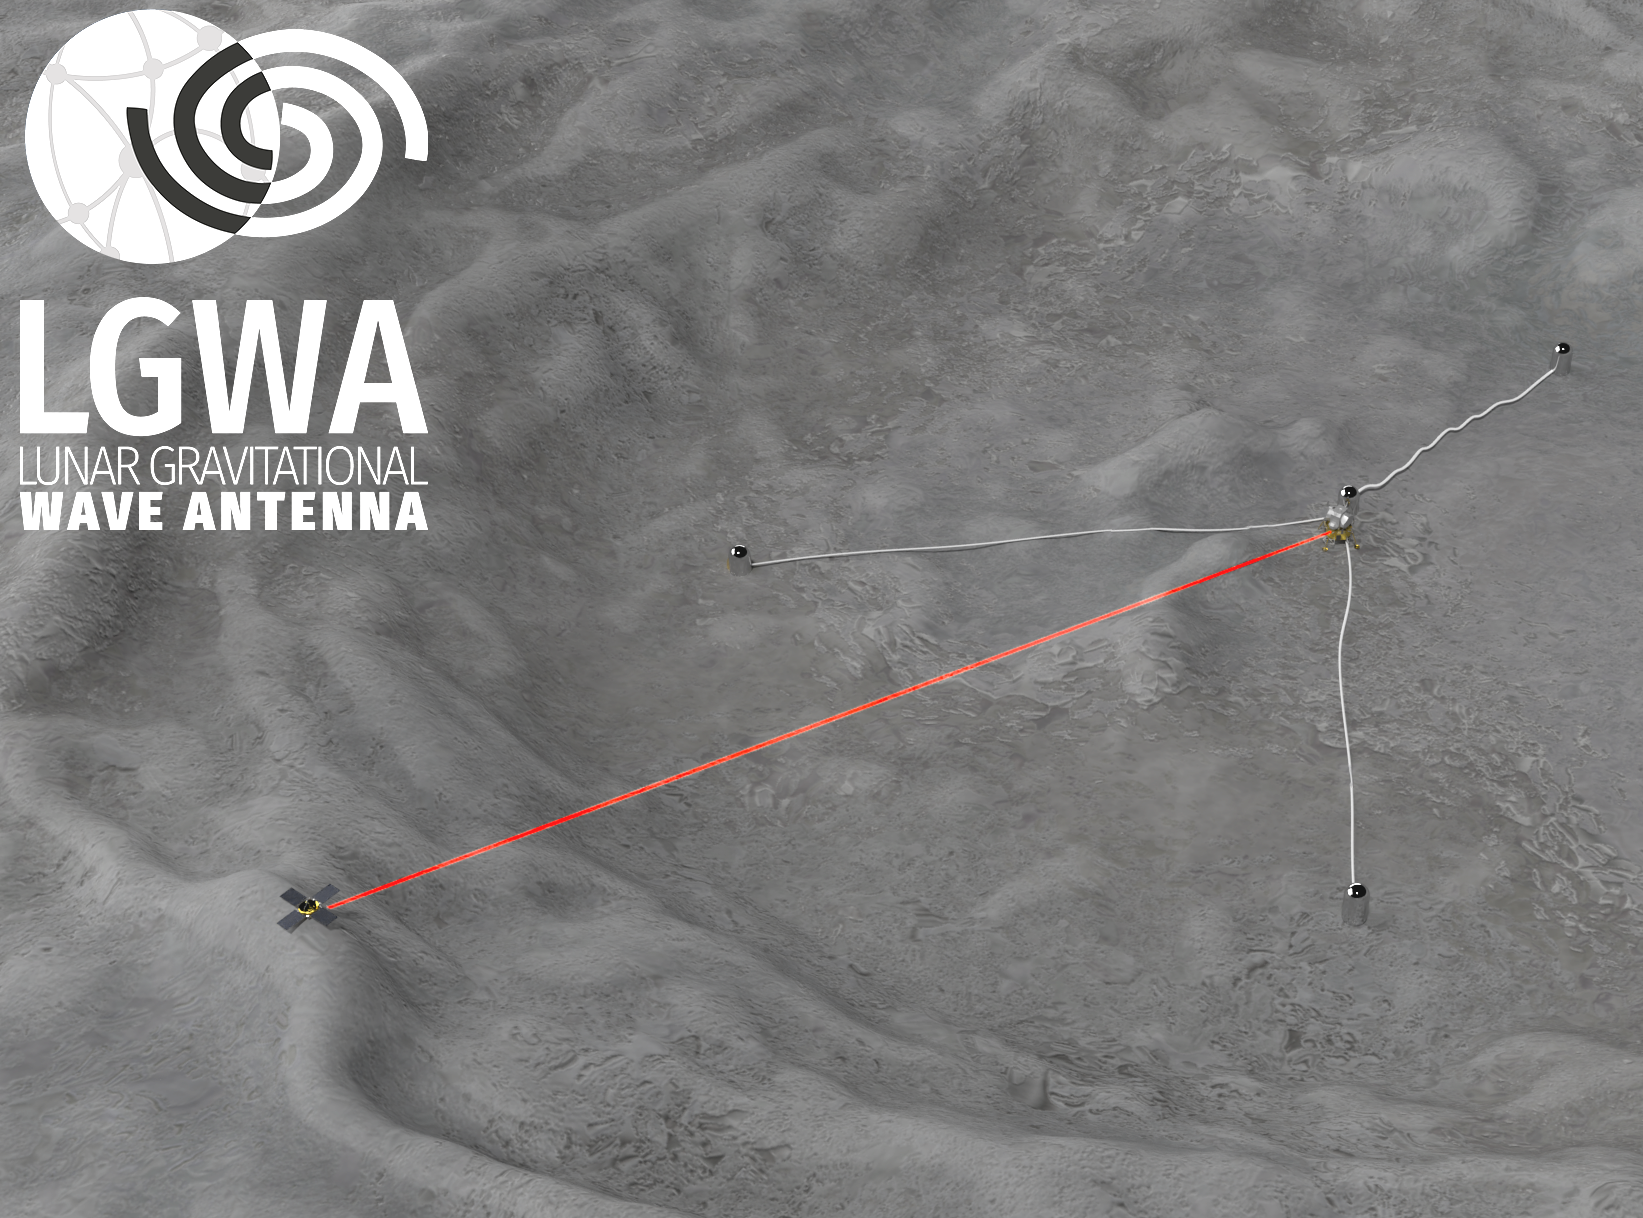
\includegraphics[width=\textwidth]{img/LGWA_crater_lighter.png}
    %%%% Bottom space

\vspace{10mm}
\Large{$^*$: A BNS system with parameters set to the median values of GW170817. This is an optimistic scenario: a "golden binary" at \(\sim\)~40 Mpc; while the BNS horizon for LGWA is roughly 180Mpc.}
% \vspace{}

%% QR code and other stuff
% \qrcode{img/qrcode}{img/smartphoneWhite}{
% \textbf{Take a picture} to
% \\ learn more details
% }
% Smartphone icon
% Author: Freepik
% Retrieved from: https://www.flaticon.com/free-icon/smartphone_65680

%% Compact QR code (comment the previous command and uncomment this one to switch)

}

}{
%%%%%%%% LEFT COLUMN

\title{Multi-banding with LGWA}
\author{Jacopo Tissino}
\author{Supervisor: Jan Harms}
\vspace{5mm}
\institution{Gran Sasso Science Institute}

\vspace{10mm}
\section{Detector concept}
\vspace{-1cm}

\begin{itemize}
    \item A \textbf{deci-hertz} GW detector
    \item Inertial sensing of \textbf{seismic motion}
    \item The lunar seismic background is much quieter than the Earth's
    \item \text{Permanently shadowed region} at the pole, $T\sim 40 \text{K}$
    \item \textbf{Cryogenic} operation at $T\sim 4 \text{K}$
    \item \textbf{SQUID} or interferometric readout
\end{itemize}

\vspace{20mm}
\section{Science targets}
\vspace{-1cm}

\begin{itemize}
    \item \textbf{Multibanding} for BNS (and BBH)
    \item \textbf{Intermediate mass} BBH (horizon at \(z \gtrsim 10\) for $10^3 M_{\odot} \lesssim M \lesssim 10^4 M_{\odot}$)
    \item Extreme and \textbf{intermediate mass ratio} inspirals
    \item NS-\textbf{white dwarf} and double white dwarf binaries
    \item \textbf{lunar science}: formation history, geologic models\dots
\end{itemize}

\vspace{20mm}
\section{Forecasting}
\vspace{-1cm}

The ingredients for our estimates:
\begin{itemize}
    \item Inertial sensing \textbf{sensitivity} estimates
    \item Lunar \textbf{response} to GWs
    \item Seismic \textbf{background} model
    \item Fisher matrix approach (assuming a matched-filtering search)
    \item Moon motion
\end{itemize}

%% This fills the space between the content and the logo
\vfill
All work within this poster is preliminary.
The LGWA collaboration is writing the whitepaper in these months.
The mission is planned for the 2030s.
\vspace{5mm}

%% Institution logo
\begin{center}
    
\includegraphics[width=.8\textwidth]{img/logo-gssi-new.png}\\
\end{center}

}{
%%%%%%%% RIGHT COLUMN
\section{Detector noise model}
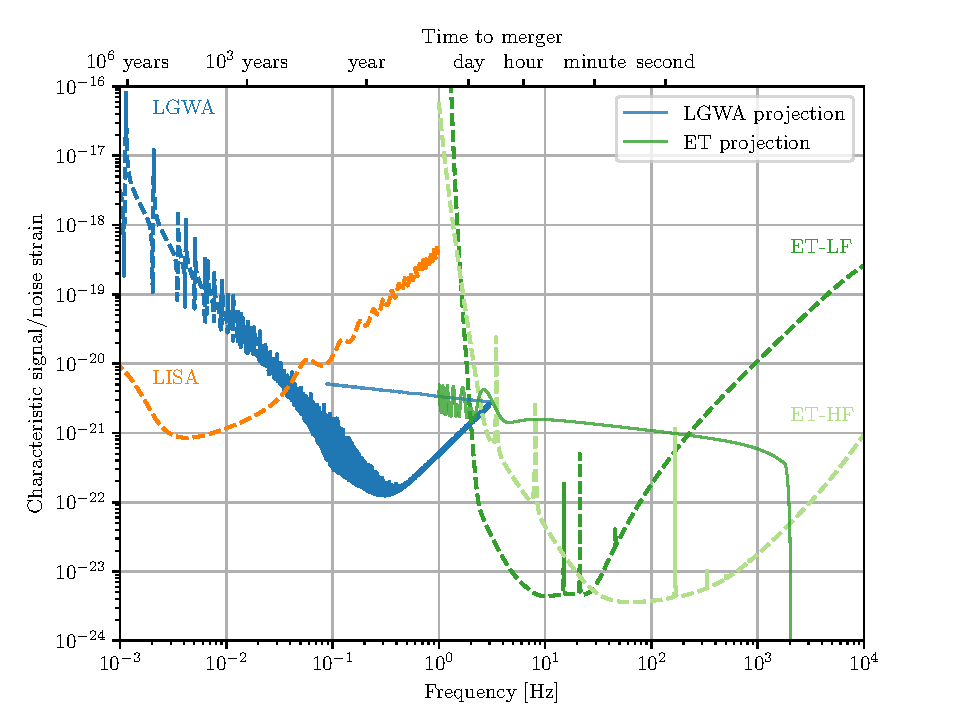
\includegraphics[width=\textwidth]{../plots/sensitivity_curves.pdf}
\section{SNR accumulation}
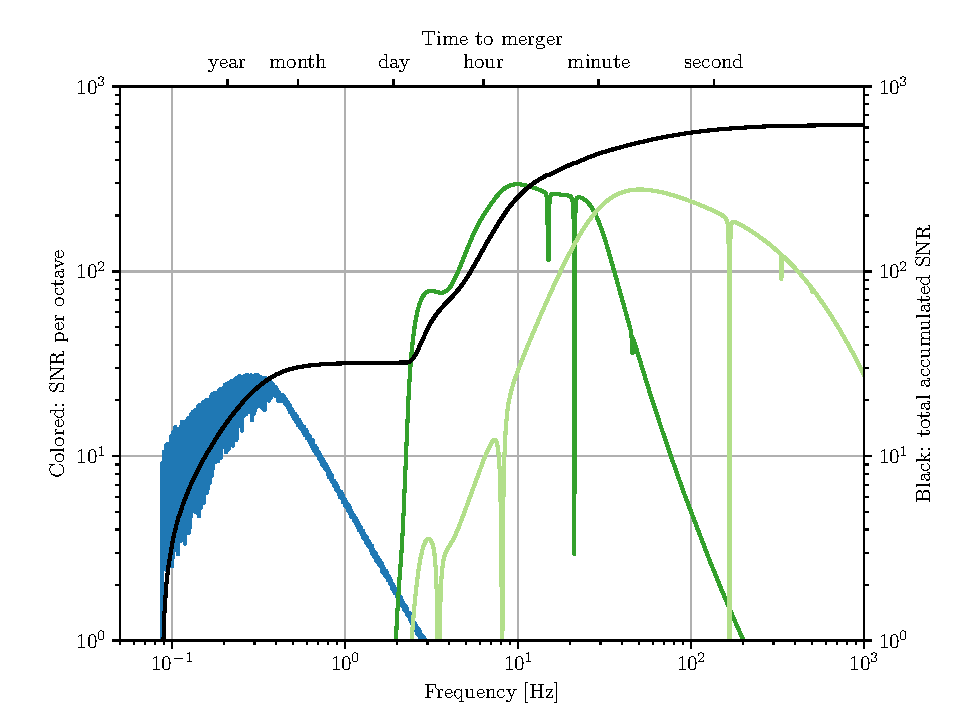
\includegraphics[width=\textwidth]{../plots/snr_integrand.pdf}
\section{Sky localization}
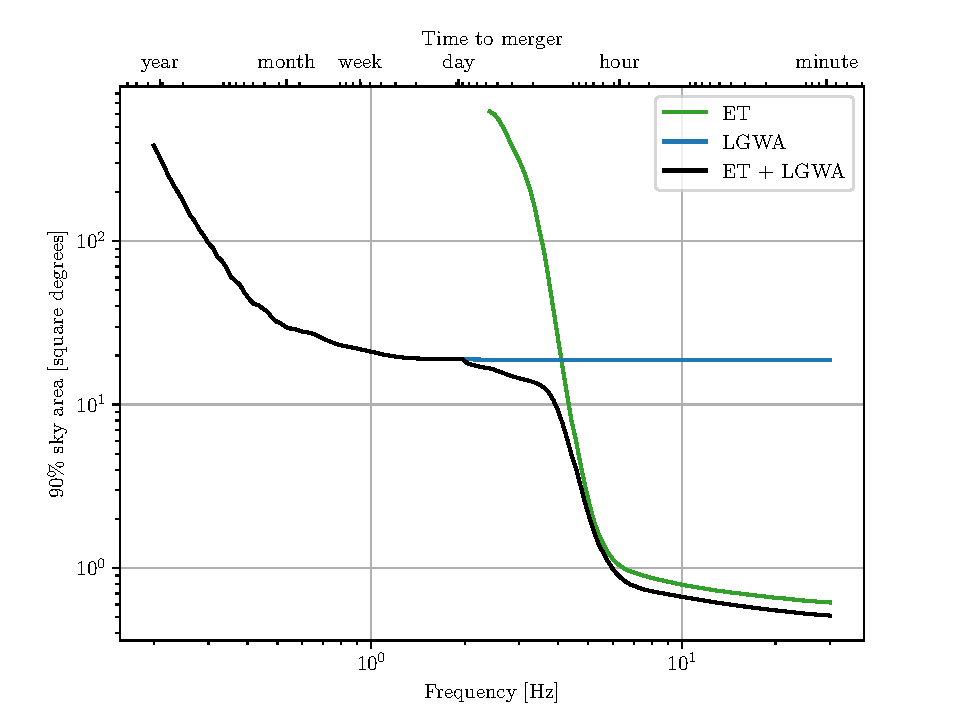
\includegraphics[width=\textwidth]{../plots/localizations.pdf}
    

}
\end{document}